% TRUST-BIO manuscript, first full draft (2026-09-29), written to the conventions of
% pisces-rct/docs/v2paper/main.tex (ML4H 2026 proceedings, jmlr class).
% Every number is taken from results/full_transport.csv, results/full_bench_*.csv,
% results/taxonomy/ and results/stress/ (see README run records). Non-rendering
% AUTHOR TODO comments mark residual work; \placeholder{} marks text the authors must supply.
% AUTHOR TODO FIGURE 1: study-overview figure does not exist yet; a framed placeholder is typeset in its place.
% AUTHOR TODO CITATIONS: bib keys marked [VERIFY] in ref.bib carry placeholder author fields; check every entry against the publisher record before submission.
\documentclass[pmlr,twocolumn,10pt]{jmlr}

\mlhtrack{proceedings}

\newif\iffinal
\finalfalse  % toggle for camera-ready

\iffinal
    \ifmlhneedspmlr
      \jmlrvolume{XXX}
      \jmlryear{2026}
    \fi
    \jmlrworkshop{Machine Learning for Health (ML4H) 2026}
\else
    \jmlrproceedings{}{Submitted to ML4H 2026: \mlhtrackname}
    \jmlrworkshop{Machine Learning for Health (ML4H) 2026}
\fi

\urlstyle{same}
\usepackage{booktabs}
\usepackage{array}
\usepackage{enumitem}
\usepackage{xcolor}
\usepackage{siunitx}
\usepackage[switch]{lineno}
\usepackage{float}
\makeatletter\setlength{\@fptop}{0pt}\makeatother
\newcommand{\placeholder}[1]{\textcolor{red}{[#1]}}
\newcommand{\domainmodel}{xECG}
\newcommand{\tsmodel}{MOMENT}

\iffinal
  \title[Biosignal Foundation-Model Stress Test]{Cross-Institution Transport and
  Sensor-Fault Stress Test of Biosignal Foundation Models}
\else
  \title[Biosignal Foundation-Model Stress Test]{Cross-Institution Transport and
  Sensor-Fault Stress Test of Biosignal Foundation Models}
\fi

% AUTHOR TODO AUTHORS: confirm the author list and affiliations before toggling \finaltrue.
\iffinal
  \author{%
   \Name{Manan Pancholy} \Email{manan\_pancholy@hms.harvard.edu}\\
   \addr Brown University, Providence, RI, USA \\
         Department of Biomedical Informatics, Harvard Medical School,
         Boston, MA, USA
   \AND
   \Name{Pranav Rajpurkar} \Email{pranav\_rajpurkar@hms.harvard.edu}\\
   \addr Department of Biomedical Informatics, Harvard Medical School,
         Boston, MA, USA
  }
\else
  \author{Anonymous Author(s)}
\fi

\renewcommand{\dbltopfraction}{0.92}
\renewcommand{\dblfloatpagefraction}{0.7}
\renewcommand{\topfraction}{0.9}
\renewcommand{\textfraction}{0.08}
\setcounter{dbltopnumber}{2}
\setcounter{topnumber}{3}
\setcounter{totalnumber}{5}

\linenumbers % remove for camera-ready

\begin{document}

\maketitle

\ifmlhdemo\else
\begin{abstract}
Foundation models for physiological waveforms are benchmarked at single sites on clean signals, and deployment adds a second site and degraded sensors. We test whether a single-site ranking of biosignal foundation models transports to an independent institution and survives injected sensor faults, and whether the faults that hurt can be detected without labels. We evaluate four domain-specific models, two general time-series models, and a hand-crafted feature baseline as frozen encoders with linear probes for heart rate and blood pressure on PulseDB, whose 5,361 subjects are partitioned by source institution, and we inject motion artifact and electrode dropout at three severities anchored to the noise of real smartphone recordings. The seven-model ranking is nearly identical at the two institutions (Spearman 0.97), but the reported ordering of model classes holds at neither: one domain model ranks first and both general models rank above the other three domain models. Heart rate transports and blood pressure does not. Motion artifact at the median and 75th-percentile noise of real recordings leaves the probes unharmed, and a signal-quality rule catches all of the harm done at the 95th percentile. Electrode dropout harms from a one-second flat-line, reorders the models, and evades the same rule below three seconds, a resolution limit of the detector rather than of the signal. Cross-institution shift leaves no label-free fingerprint. The faults a label-free quality index misses are the ones that do not hurt, with one repairable exception.
\end{abstract}
\begin{keywords}
foundation models, electrocardiography, photoplethysmography, distribution shift,
signal quality, robustness
\end{keywords}
\fi

\ifmlhneedsstatements
\paragraph*{Data and Code Availability}
This study uses three public datasets. PulseDB is distributed by its authors under their original terms \citep{wang2023pulsedb}. MIMIC-III-Ext-PPG is distributed on PhysioNet under the PhysioNet Credentialed Health Data License and was accessed by credentialed authors who completed the required training and data use agreement \citep{mimicextppg,goldberger2000physionet}. BUT PPG is distributed under a Creative Commons Attribution 4.0 license \citep{nemcova2021butppg}. Model weights are those released by their authors. The feature store, degradation injection, probes, fault taxonomy, and every table and figure in this paper are produced by the pipeline described in \sectionref{sec:methods}; code will be released upon acceptance.

\paragraph*{Institutional Review Board (IRB)}
This research does not require IRB approval; \iffinal Harvard Medical School\else the authors' institution\fi{} determined that it does not constitute human-subjects research. It is a secondary analysis of de-identified, previously collected public datasets, each governed by its originating institution's ethics approval and data use terms. No new human-subjects data were collected.
\fi

\section{Introduction}
\label{sec:intro}

Foundation models pretrained on electrocardiogram (ECG) and photoplethysmogram (PPG) corpora are used as frozen encoders whose embeddings feed light task-specific probes \citep{goswami2024moment,ansari2024chronos,li2024ecgfounder,pillai2024papagei}. They are evaluated by holding out patients within one source institution, and a recent single-site benchmark of this kind, SignalMC-MED, reported that domain-specific biosignal models outperform general time-series models and that ECG+PPG fusion adds to the better single modality \citep{signalmcmed}. Deployment differs from that evaluation in two ways: a second institution brings its own population and monitors, and a worn or handled sensor brings motion artifact, electrode dropout, and missing channels. Rankings of clinical models measured at one site have been found to encode that site's acquisition artifacts \citep{zech2018variable,finlayson2021clinician}.

Signal degradation is not one problem. A window can be untrustworthy because of a brief burst of motion, a persistently disconnected electrode, or a systematic difference between the deployment device and population and those seen in pretraining. Fault-tolerant sensor systems treat transient and structural faults separately because they call for different responses: the first is waited out, the second requires adaptation or abstention \placeholder{CITE: fault taxonomy in fault-tolerant sensor fusion}. Whether these classes can be told apart without diagnostic labels, and whether the classes that cannot be detected are the ones that harm a model, determines what a fault-aware system can achieve.

We answer three questions on the same cohort. First, does the single-site ordering of model classes transport to an independent, cross-institution cohort? Second, how does the ordering change under controlled degradation, and how much of the resulting harm does a label-free signal-quality index catch? Third, do degraded and shifted windows fall into transient, persistent, and structural classes without labels? We use PulseDB, whose 5,361 subjects are partitioned by source institution into a Boston intensive-care cohort and a Seoul surgical cohort \citep{wang2023pulsedb,johnson2016mimic,lee2022vitaldb}, MIMIC-III-Ext-PPG for its native signal-quality codes \citep{mimicextppg}, and BUT PPG, a smartphone-camera PPG database with a human quality label, as the source of real degradation \citep{nemcova2021butppg}. Seven encoders are compared through the same linear-probe protocol: \domainmodel{}, ECGFounder, PaPaGei, and D-BETA as domain-specific models, \tsmodel{} and Chronos-Bolt as general time-series models, and NeuroKit2 features as a hand-crafted baseline. Our contributions are as follows.
\begin{itemize}[leftmargin=*,itemsep=2pt,topsep=3pt]
\item \textbf{We show that a single-site ranking transports across institutions but the class-level claim built on it does not.} The seven-model ranking has Spearman correlation 0.97 between the two institutions, yet one domain model ranks first and both general models rank above the other three domain models at both sites. Heart-rate probes keep most of their within-site score across institutions and blood-pressure probes do not.
\item \textbf{We show that realistic motion artifact does not harm the probes and that the harm it does at the extreme is fully caught without labels.} Motion noise at the median and 75th-percentile level of real smartphone recordings moves 0.1\% and 2.7\% of heart-rate estimates by more than 5 beats per minute; at the 95th-percentile level it moves 58\%, and a per-second quality rule flags every affected window.
\item \textbf{We show that electrode dropout is the fault that both harms and hides.} A one-second flat-line moves 26\% of heart-rate estimates by more than 5 beats per minute, reorders the models, and is flagged in 2\% of windows by the same rule, because the rule's one-second bins straddle a one-second span. This is a detector-resolution limit, and it names the repair.
\item \textbf{We show that label-free clustering recovers only severe faults, that supervision recovers moderate ones, and that cross-institution shift has no signal-quality or model-disagreement fingerprint.} Clean windows from the second institution are indistinguishable from clean windows of the first (out-of-fold AUROC 0.68), which bounds what any quality index can flag before a site-level calibration sample exists.
\end{itemize}

\section{The Single-Site Claim and the Cohort}
\label{sec:claim}

SignalMC-MED compared domain-specific biosignal foundation models, general time-series foundation models, and ECG+PPG fusion on patients held out within one emergency department, and reported that the domain-specific models rank higher and that fusion adds to the better single modality \citep{signalmcmed}. The claim concerns model classes rather than individual checkpoints, and it was measured on one site's monitors, population, and signal quality.

PulseDB supplies a cohort on which the claim can be re-measured across institutions \citep{wang2023pulsedb}. It contains 10-second windows of synchronized ECG, PPG, and arterial blood pressure at \SI{125}{\hertz}, retained as two partitions by source database: PulseDB-MIMIC, derived from the MIMIC-III Waveform Database Matched Subset collected in Boston intensive-care units \citep{johnson2016mimic}, and PulseDB-Vital, derived from VitalDB collected in Seoul operating rooms \citep{lee2022vitaldb}. The partition is the transport axis of this study: a probe fit on one institution is scored zero-shot on the other. PulseDB's arterial channel provides per-window systolic and diastolic blood pressure, and heart rate is derived from each window's ECG. The three tasks common to the cohorts, heart rate, systolic pressure, and diastolic pressure, are the tasks we evaluate.

\section{Methods}
\label{sec:methods}

The study comprises four components (\figureref{fig:overview}): a feature store of frozen-encoder embeddings for every 10-second window of both PulseDB institutions; a linear-probe protocol applied within and across institutions; a degradation stress test in which the same windows are embedded clean and under injected faults, so that harm is measured per window; and a label-free fault taxonomy whose detection rules are joined to that harm. The following subsections describe each component. \sectionref{sec:stats} states the statistical conventions.

\begin{figure*}[t]
\floatconts
  {fig:overview}
  {\caption{Study design. Seven frozen encoders embed 10-second ECG and PPG windows from two PulseDB institutions, MIMIC-III-Ext-PPG, and BUT PPG. Linear probes for heart rate and blood pressure are fit on one institution and scored on the other. The same windows are re-embedded under injected motion artifact and electrode dropout at three severities, giving paired predictions from which per-window harm is measured. Per-second signal-quality traces computed on the identical corrupted waveforms feed a label-free fault taxonomy whose detection rules are then joined to the harm. \placeholder{FIGURE NEEDED: study-overview schematic}}}
  {\fbox{\parbox{0.96\linewidth}{\centering\vspace{1.2cm}\placeholder{Figure 1 placeholder: study-overview schematic to be drawn}\vspace{1.2cm}}}}
\end{figure*}

\subsection{Datasets}
\label{sec:data}

\paragraph{PulseDB.}
We build one visit per window that passes PulseDB's native inclusion flag, with all windows of a subject assigned to the same split: 3,791,004 windows from 2,423 subjects for PulseDB-MIMIC (train 2,691,120, validation 577,755, test 522,129 windows; 1,696, 363, and 364 subjects) and 1,454,450 windows from 2,938 subjects for PulseDB-Vital (1,019,397, 208,844, and 226,209 windows; 2,057, 441, and 440 subjects). Splits are random at the subject level in a 70/15/15 ratio. Systolic and diastolic labels are the per-window values PulseDB derives from the arterial channel. Heart rate is estimated from each window's ECG by QRS detection in a 5--15~\si{\hertz} band with a prominence threshold and the median of physiologically plausible inter-beat intervals; against BUT PPG's 400 human-annotated good-quality records the estimator has a mean absolute error of 1.0 beats per minute and a correlation of 0.94 with the reference, and against PulseDB's own arterial pulse rate a correlation of 0.99. The estimate is undefined for 4 MIMIC and 98 Vital windows, which are excluded from the heart-rate task. Median labels are 85.2 and 76.5 beats per minute, 121.9 and 114.0~\si{\milli\meter Hg} systolic, and 60.1 and 62.0~\si{\milli\meter Hg} diastolic for MIMIC and Vital, respectively.

\paragraph{MIMIC-III-Ext-PPG.}
This database provides 30-second PPG and ECG segments from intensive-care patients with a native per-10-second signal-quality code for each channel \citep{mimicextppg}. We sample 2,400 segments from 1,512 subjects, at most 4 per subject, stratified by the native codes of the first 10 seconds: 800 with both channels coded clean, 800 with the PPG coded poor, and 800 with the PPG coded clean and the ECG coded poor or missing. These strata serve as held-out real-degradation groups and as the validation set for our own quality traces. Heart-rate labels are the database's median 30-second heart rate. MIMIC-III-Ext-PPG derives from the same Boston waveform database as PulseDB-MIMIC, so it is a second acquisition pipeline rather than a second institution.

\paragraph{BUT PPG.}
The Brno University of Technology smartphone PPG database contains 3,888 10-second smartphone-camera PPG recordings at \SI{30}{\hertz} from 50 subjects, with a reference ECG, triaxial accelerometry for the later records, and a binary human annotation of usability for heart-rate estimation \citep{nemcova2021butppg}. We retain all 3,888 recordings, including 48 whose headers are malformed upstream and whose waveforms we reconstruct from the header gain fields; excluding them would remove 12 of 50 subjects. By the native label, 830 recordings are usable and 3,058 are not. BUT PPG supplies the real noise distribution against which synthetic motion artifact is calibrated and a held-out real-degradation group.

\subsection{Encoders and feature extraction}
\label{sec:models}

We compare seven encoders as frozen feature extractors, with no fine-tuning (\tableref{tab:models}). Four are domain-specific: \domainmodel{}, an xLSTM ECG model whose long-input variant we use \placeholder{CITE: xECG}; ECGFounder, a single-lead ECG model \citep{li2024ecgfounder}; PaPaGei-S, a PPG model \citep{pillai2024papagei}; and D-BETA, an ECG model \placeholder{CITE: D-BETA}. Two are general time-series models, \tsmodel{}-base \citep{goswami2024moment} and Chronos-Bolt-small \citep{ansari2024chronos}. The seventh is a hand-crafted baseline of 54 NeuroKit2 ECG features \citep{makowski2021neurokit}. Each encoder is applied to both modalities: every model receives the ECG window and, separately, the PPG window, whichever modality it was pretrained on, so that a PPG model's ECG embedding and an ECG model's PPG embedding are evaluated like any other. Each window is resampled to the encoder's expected rate, cleaned and z-normalized, encoded, and mean-pooled to one vector per modality. The fusion vector is the element-wise mean of the ECG and PPG vectors, following the single-site benchmark. Extraction runs on the full PulseDB cohorts in chunked, resumable batch jobs, and every stored cell is verified for row count and cohort order before evaluation.

\begin{table}[t]
\floatconts
  {tab:models}%
  {\caption{Encoders. Parameters and embedding dimension are those of the released checkpoints; the NeuroKit2 baseline is a fixed feature set.}}%
  {\footnotesize\setlength{\tabcolsep}{3pt}
  \begin{tabular*}{\linewidth}{@{\extracolsep{\fill}}llrr@{}}
  \toprule
  \textbf{Encoder} & \textbf{Class} & \textbf{Params} & \textbf{Dim.} \\
  \midrule
  \domainmodel{} (10-min variant) & domain, ECG & 57M & 1024 \\
  ECGFounder (single lead) & domain, ECG & 31M & 1024 \\
  D-BETA & domain, ECG & 62M & 768 \\
  PaPaGei-S & domain, PPG & 6M & 512 \\
  \tsmodel{}-base & general time series & 110M & 768 \\
  Chronos-Bolt-small & general time series & 48M & 512 \\
  NeuroKit2 ECG features & hand-crafted & -- & 54 \\
  \bottomrule
  \end{tabular*}}
\end{table}

\subsection{Linear probes within and across institutions}
\label{sec:probes}

Every task is a ridge regression on the standardized embedding, scored by Pearson correlation between predicted and true values, following the single-site benchmark's protocol \citep{signalmcmed,pedregosa2011sklearn}. One regularization strength per encoder, modality, and institution is chosen from a grid of 31 values between $10^{-6}$ and $10^{6}$ by heart-rate correlation on the validation split, then frozen for all three tasks.

\paragraph{Within-institution benchmark.}
Within each institution the probe is fit on the train split and scored on the test split, with the train split resampled with replacement at 10\%, 25\%, 50\%, and 100\% of its visits over 5 repeats; the reported score is the mean over fractions and repeats, and blood pressure is the mean of the systolic and diastolic scores. Models are ranked within each task category and the ranks averaged, separately per institution.

\paragraph{Cross-institution transport.}
The probe is fit on the full train split of the source institution, its regularization chosen on the source validation split, and it is scored zero-shot on all windows of the target institution, in both directions. No target data enter the fit.

\subsection{Degradation injection}
\label{sec:degradation}

We inject three faults into the raw waveform before any encoder preprocessing, each on a contiguous span covering a fraction of the window that we call severity, at severities 0.1, 0.3, and 0.6. Motion artifact adds smoothed white noise to the PPG span; electrode dropout, or lead-off, sets the ECG span to zero; missing PPG removes the PPG channel, which for the fusion probe means the ECG vector is used alone. Each fault therefore touches one modality, so an ECG probe under motion and a PPG probe under lead-off see embeddings identical to the clean ones. The corrupted span and the noise are a deterministic function of the window identifier and the condition, so the taxonomy can recompute the exact waveform a model was fed.

\paragraph{Calibration to real noise.}
The original design mapped severity to a fraction of the accelerometer range in BUT PPG. On the real data no such relationship exists: accelerometer dynamics separate usable from unusable recordings with an area under the receiver operating characteristic curve (AUROC) of 0.57, and the Spearman correlation between accelerometer magnitude and PPG noise is $-0.11$ over 3,795 accelerometer-era recordings. We report this as a negative result and instead anchor each severity to a quantile of real smartphone-PPG noise. The noise statistic is the ratio of the standard deviation of the residual above an 8~\si{\hertz} low-pass filter to that of the signal, which means the same thing at \SI{30}{\hertz} and \SI{125}{\hertz}. Over 3,843 BUT PPG recordings its 50th, 75th, and 95th percentiles are 0.057, 0.091, and 0.318. For each severity we solve by bisection, on 200 clean PulseDB reference windows, for the noise amplitude that reproduces the corresponding percentile within the corrupted span, obtaining 0.18, 0.31, and 1.30 times the signal's standard deviation. A severity-0.6 window is therefore as noisy, over 60\% of its length, as the noisiest 5\% of real smartphone seconds.

\subsection{Stress test on paired predictions}
\label{sec:stress}

The stress test asks what a fault does to a probe's prediction on the same window. We draw a stress cohort of 60 subjects per institution with at most 40 windows each, 1,980 windows from PulseDB-MIMIC and 2,093 from PulseDB-Vital, and the 2,400 MIMIC-III-Ext-PPG segments, and embed every window with every encoder under the clean condition and each of the six injected conditions, 1,386 verified store cells in all. Probes are refit exactly as in \sectionref{sec:probes} on each institution's full train split with the 60 stress-cohort subjects removed, so that within-institution scores are held-out-subject scores, and applied to every condition of both PulseDB targets and to MIMIC-III-Ext-PPG for heart rate. This yields 4,502,652 paired predictions. Harm on a window is the absolute error under the fault minus the absolute error under the clean condition, for the same probe. A window is materially harmed when its estimate moves by more than 5 beats per minute or 5~\si{\milli\meter Hg}. We summarize each encoder, modality, source, target, and condition by its correlation, its mean absolute error, and the change in each from the clean baseline, and we average over the seven encoders and the four source--target pairs where the text says so. Ranking stability is the Spearman correlation between the seven encoders' clean scores and their scores under a condition. Fusion is compared with the better of its two unimodal probes under the same condition; under missing PPG the comparator is the clean ECG probe.

\subsection{Label-free fault taxonomy}
\label{sec:taxonomy}

The taxonomy asks whether degraded and shifted windows fall into transient, persistent, and structural classes without diagnostic labels. It is built on the identical corrupted waveforms the encoders received, for every window of the stress cohort under every condition, plus the clean BUT PPG recordings: 49,199 rows in all.

\paragraph{Quality traces.}
Each window receives a per-second quality trace per modality. The ECG trace is an electrode-off detector: a one-second bin whose spread is below $10^{-4}$ of the whole window's spread scores 0, and every other bin scores 1. A noise-based ECG measure is backwards, because QRS complexes are the high-frequency content; in the first iteration of this analysis such a measure separated natively clean from natively poor ECG with an AUROC of 0.29. The PPG trace is the out-of-band noise ratio of \sectionref{sec:degradation} per second, mapped to quality as $1-\text{ratio}/\text{ref}$ clipped to $[0,1]$, where the reference 0.375 is the 95th percentile of 38,870 real BUT PPG seconds; a flat second scores 0. The combined trace is the per-second minimum. Against MIMIC-III-Ext-PPG's native codes on the clean condition, the PPG trace separates poor from clean segments with an AUROC of 0.65 ($n=2{,}400$) and the ECG trace with 0.51 ($n=1{,}600$); the native ECG code marks missing samples and rhythm-annotation failures rather than flat-lines, and we do not tune the traces to it.

\paragraph{Features.}
Nine features describe each window: the combined mean quality and longest low-quality run, the same two per modality, the correlation between the low-quality indicator and accelerometer magnitude where an accelerometer exists, the source database, and a model-disagreement statistic. The disagreement is the absolute difference between the heart-rate predictions of a \domainmodel{} probe and a \tsmodel{} probe on the fusion embedding, both fit on 500,000 clean PulseDB-MIMIC windows, divided by its spread on clean in-distribution windows. Its intended role is the structural-shift signature: two models trained on the same data disagreeing on a window whose quality looks fine. Four feature sets are evaluated: all nine features, all but the source database, all but the disagreement, and the quality features alone.

\paragraph{Clustering and validation.}
The fit set holds the synthetic motion and lead-off windows of both PulseDB institutions and MIMIC-III-Ext-PPG at all three severities, 19,419 of each kind, and the 2,093 clean PulseDB-Vital windows as the structural class, 40,931 rows. Features are standardized and clustered by $k$-means with $k=3$ \citep{pedregosa2011sklearn}. Labels are used only afterwards: each cluster takes the name of its majority known condition, and recall is the share of a condition's windows assigned to a cluster carrying its name, with 95\% confidence intervals from 200 bootstrap resamples of subjects. Clean PulseDB-MIMIC windows, the three MIMIC-III-Ext-PPG strata, and BUT PPG's usable and unusable recordings are held out and assigned to the nearest centroid. Two further analyses bound the clustering. A supervised ceiling fits logistic regression and gradient-boosted trees on the same rows under subject-grouped five-fold cross-validation, and a binary version separates clean Vital from clean MIMIC windows. A two-stage variant first detects degraded windows by a label-free rule, then clusters only those with $k$ chosen from 2 to 6 by silhouette on a 5,000-row subsample \citep{rousseeuw1987silhouette}. Two rules are used: the drop rule flags a window whose combined trace falls below 0.5 for at least one second, and the outlier rule flags a window whose PPG or ECG quality lies below the 2.5th percentile, or whose disagreement lies above the 97.5th percentile, of the clean PulseDB-MIMIC controls. A supervised detector, gradient-boosted trees fit out of fold on synthetic rows versus clean controls, gives the detection ceiling.

\subsection{Statistical analysis}
\label{sec:stats}

Probe scores are Pearson correlations; transport and stress comparisons are descriptive and no hypothesis test is applied to a difference between two scores. Recall intervals are subject-clustered bootstrap 95\% intervals, because windows of one subject are not independent. Ranking agreement is Spearman's rank correlation over the seven encoders. Harm coverage is reported two ways: the share of the summed positive harm that falls in flagged windows, and the fraction of materially harmed windows that are flagged. Where a mean is taken over encoders and source--target pairs, the number of cells averaged is stated.

\section{Results}
\label{sec:results}

\subsection{The ranking transports across institutions, but the class-level claim does not}
\label{sec:transport}

The order in which the seven encoders rank is the same at the two institutions, and it is not the order the single-site claim predicts (\tableref{tab:transport}). Mean ranks across the heart-rate and blood-pressure categories have Spearman correlation 0.97 between Boston and Seoul, and the within-institution heart-rate scores alone have correlation 0.96. \domainmodel{} ranks first at both institutions with heart-rate correlations of 0.83 and 0.79. The two general time-series models rank second and third in Boston and second and equal-third in Seoul, above PaPaGei and D-BETA at both institutions and above ECGFounder in Boston. The hand-crafted baseline ranks last at both. The single-site ordering of classes, domain above general, therefore describes one checkpoint rather than a class: three of the four domain-specific encoders rank below one or both general models at both institutions.

Cross-institution scores follow the same order. Fit on Boston and scored on Seoul, the fusion probes' heart-rate correlations run from 0.60 to 0.74 across the seven encoders, and fit on Seoul and scored on Boston from 0.65 to 0.80, with \domainmodel{} first in both directions. The full breakdown by modality is in \appendixref{apx:transport}.

\begin{table*}[t]
\floatconts
  {tab:transport}%
  {\caption{Within-institution and cross-institution probe scores (Pearson correlation) for the fusion embedding, and mean rank per institution. Within-institution scores are means over train fractions and 5 resamples of the benchmark protocol; cross-institution scores are single fits on the full source train split scored on every window of the target. Blood pressure is the mean of the systolic and diastolic scores. M, PulseDB-MIMIC (Boston); V, PulseDB-Vital (Seoul); M$\to$V, fit on Boston and scored on Seoul.}}%
  {\footnotesize\setlength{\tabcolsep}{3pt}
  \begin{tabular*}{\linewidth}{@{\extracolsep{\fill}}lcccccccccc@{}}
  \toprule
  & \multicolumn{4}{c}{\textbf{Heart rate}} & \multicolumn{4}{c}{\textbf{Blood pressure}} & \multicolumn{2}{c}{\textbf{Mean rank}} \\
  \cmidrule(lr){2-5}\cmidrule(lr){6-9}\cmidrule(lr){10-11}
  \textbf{Encoder} & within M & within V & M$\to$V & V$\to$M & within M & within V & M$\to$V & V$\to$M & M & V \\
  \midrule
  \domainmodel{} & 0.83 & 0.79 & 0.74 & 0.80 & 0.45 & 0.54 & 0.38 & 0.30 & 1.0 & 1.0 \\
  \tsmodel{} & 0.82 & 0.78 & 0.70 & 0.76 & 0.33 & 0.45 & 0.31 & 0.27 & 3.0 & 2.5 \\
  Chronos-Bolt & 0.80 & 0.75 & 0.68 & 0.74 & 0.37 & 0.44 & 0.31 & 0.28 & 3.0 & 3.5 \\
  ECGFounder & 0.77 & 0.72 & 0.63 & 0.70 & 0.43 & 0.51 & 0.36 & 0.31 & 4.0 & 3.5 \\
  PaPaGei & 0.79 & 0.75 & 0.69 & 0.75 & 0.27 & 0.30 & 0.21 & 0.21 & 4.5 & 5.0 \\
  D-BETA & 0.77 & 0.69 & 0.60 & 0.66 & 0.19 & 0.31 & 0.28 & 0.20 & 5.5 & 5.5 \\
  NeuroKit2 features & 0.71 & 0.63 & 0.60 & 0.65 & 0.16 & 0.20 & 0.07 & 0.09 & 7.0 & 7.0 \\
  \bottomrule
  \end{tabular*}}
\end{table*}

\subsection{Heart rate transports across institutions and blood pressure does not}
\label{sec:tasks}

Heart-rate probes keep most of their score at the other institution and blood-pressure probes lose most of theirs. From the ECG embedding, the six foundation models' heart-rate correlations are 0.61 to 0.75 when fit on Boston and scored on Seoul, and 0.65 to 0.80 in the reverse direction, against within-institution fusion scores of 0.69 to 0.83. Blood pressure from the ECG embedding falls to a mean correlation of 0.10 and 0.14 in the two directions, from the PPG embedding to 0.36 and 0.31, and from fusion to 0.31 and 0.26, against within-institution scores of 0.19 to 0.45 in Boston and 0.30 to 0.54 in Seoul.

One transport failure is shared by every encoder and belongs to the data rather than to a model. Heart rate from the PPG embedding, fit on Boston and scored on Seoul, has a correlation of 0.32 to 0.34 for all six foundation models, while the reverse direction gives 0.65 to 0.69. The same six probes from the ECG embedding transport in both directions. A model-independent, modality-specific loss of this kind is the signature of a difference in the PPG acquisition or population between the two institutions, and it is the structural class that \sectionref{sec:taxonomy_results} tests for.

\subsection{Mean fusion never beats the better single modality}
\label{sec:fusion}

Averaging the ECG and PPG embeddings does not add to the better of the two, within or across institutions, clean or degraded. Across the 42 cross-institution cells of encoder, direction, and task, the fusion probe scores above the better unimodal probe in 6, and its mean shortfall is 0.02 for heart rate and 0.04 to 0.06 for blood pressure (\appendixref{apx:transport}). In the stress test, averaged over the seven encoders and four source--target pairs, the fusion heart-rate probe scores 0.01 below the better unimodal probe on clean windows, 0.02, 0.03, and 0.08 below it under lead-off at the three severities, and 0.01 to 0.02 below it under motion. Fusion cushions a fault in the corrupted modality, halving the lead-off harm of the ECG probe (\sectionref{sec:leadoff}), but at every severity the better choice is the probe on the intact modality (\figureref{fig:fusion}).

\begin{figure*}[t]
\floatconts
  {fig:fusion}
  {\caption{Fusion minus the better unimodal probe for heart rate, by injected severity, one panel per source--target pair. Each line is one encoder under motion artifact (circles) or lead-off (squares); crosses at severity 1.0 are the missing-PPG condition, in which the fusion probe receives the ECG vector. The line at zero marks parity with the better single modality.}}
  {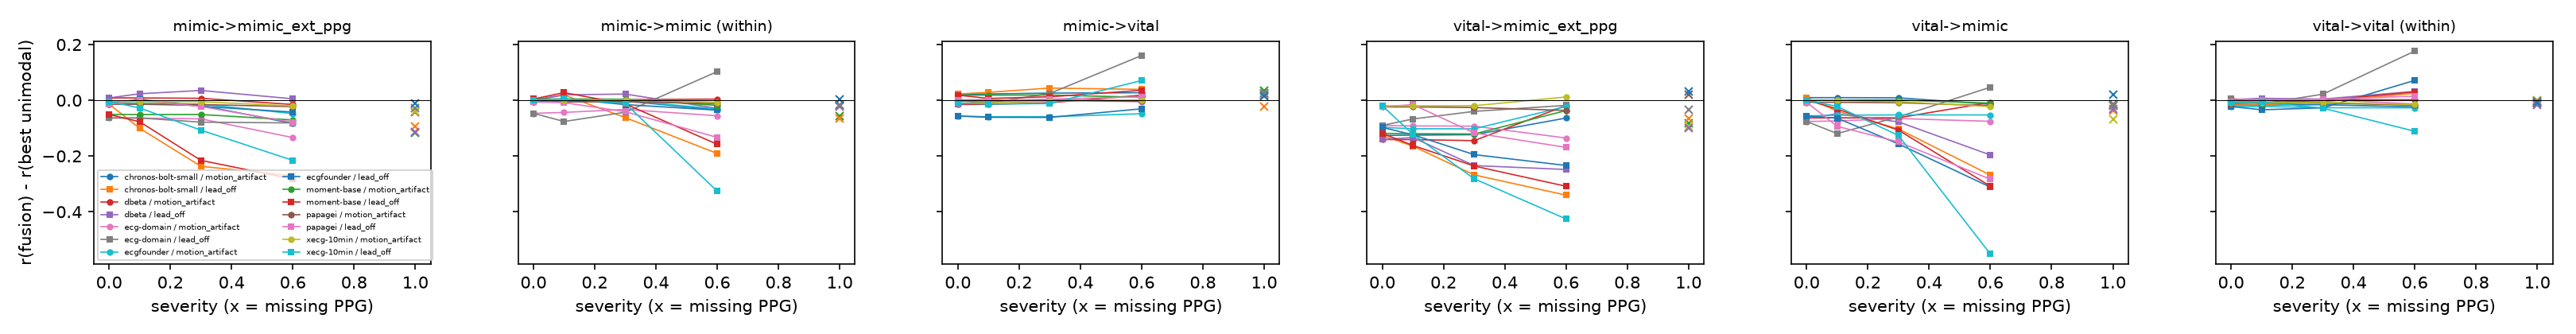
\includegraphics[width=\linewidth]{figures/fig2c_fusion_hr_regression.png}}
\end{figure*}

\subsection{Realistic motion artifact leaves the probes unharmed, and the harm at the extreme is fully caught}
\label{sec:motion}

Motion noise at the level of a typical smartphone recording does not change what the probes predict (\tableref{tab:stress}). At severities 0.1 and 0.3, the median and 75th-percentile noise of real recordings over 10\% and 30\% of the window, the PPG heart-rate probe's correlation changes by 0.000 and $+0.003$ and its mean absolute error by 0.1 and 0.6 beats per minute, averaged over 28 encoder--pair cells; 0.1\% and 2.7\% of windows move by more than 5 beats per minute. The fusion probe is unchanged. At severity 0.6, the 95th-percentile noise over 60\% of the window, the PPG probe loses 0.044 of correlation and 6.8 beats per minute of mean absolute error, with 58\% of windows moved by more than 5 beats per minute; the fusion probe loses 1.9 beats per minute with 27\% of windows moved. Blood pressure follows the same pattern: the PPG systolic probe changes by $-0.006$ at severity 0.3 and $-0.138$ at 0.6, with 5.6\% and 36\% of windows moved by more than 5~\si{\milli\meter Hg}. The MIMIC-III-Ext-PPG target reproduces the pattern, with the PPG heart-rate correlation at 0.637, 0.637, 0.636, and 0.509 across the four levels, averaged over encoders and sources.

The harm that motion does is caught without labels. The drop rule flags 100\% of severity-0.6 windows and therefore captures 100\% of the summed harm and 100\% of the materially harmed windows. At severities 0.1 and 0.3 the same rule flags 1.1\% and 1.4\% of windows, and this costs nothing because there is no harm to catch: the summed positive harm in unflagged windows is a mean of 0.1 and 0.6 beats per minute per window. The supervised detection ceiling flags 76\% of severity-0.3 windows, all of them harmless (\figureref{fig:coverage}).

\begin{table*}[t]
\floatconts
  {tab:stress}%
  {\caption{Degradation stress test for heart rate on PulseDB, averaged over the seven encoders and four source--target pairs (28 cells per row). Motion artifact corrupts the PPG channel and lead-off the ECG channel, so the affected unimodal probe and the fusion probe are shown. $\Delta r$ and $\Delta$MAE are changes from the same probe on the same windows under the clean condition; harmed is the percentage of windows whose estimate moves by more than 5 beats per minute; the last three columns give the percentage of summed positive harm that falls in windows flagged by the drop rule, the outlier rule, and the supervised detector. Missing PPG feeds the fusion probe the ECG vector and has no quality-trace counterpart.}}%
  {\footnotesize\setlength{\tabcolsep}{3pt}
  \begin{tabular*}{\linewidth}{@{\extracolsep{\fill}}llcrrrrrr@{}}
  \toprule
  & & & & & & \multicolumn{3}{c}{\textbf{Harm caught (\%)}} \\
  \cmidrule(lr){7-9}
  \textbf{Fault} & \textbf{Severity} & \textbf{Probe} & $\Delta r$ & $\Delta$\textbf{MAE (bpm)} & \textbf{Harmed (\%)} & \textbf{Drop} & \textbf{Outlier} & \textbf{Superv.} \\
  \midrule
  Motion artifact & 0.1 & PPG & $-0.000$ & $+0.1$ & 0.1 & 0.2 & 7.0 & 22.5 \\
  Motion artifact & 0.1 & Fusion & $-0.000$ & $+0.0$ & 0.2 & 0.1 & 9.6 & 22.9 \\
  Motion artifact & 0.3 & PPG & $+0.003$ & $+0.6$ & 2.7 & 1.0 & 41.4 & 80.3 \\
  Motion artifact & 0.3 & Fusion & $+0.001$ & $+0.1$ & 1.0 & 0.6 & 47.2 & 82.4 \\
  Motion artifact & 0.6 & PPG & $-0.044$ & $+6.8$ & 58.4 & 100.0 & 100.0 & 100.0 \\
  Motion artifact & 0.6 & Fusion & $-0.009$ & $+1.9$ & 26.8 & 100.0 & 100.0 & 100.0 \\
  \midrule
  Lead-off & 0.1 & ECG & $-0.032$ & $+1.5$ & 26.0 & 0.8 & 8.9 & 14.4 \\
  Lead-off & 0.1 & Fusion & $-0.032$ & $+1.1$ & 20.3 & 0.9 & 9.1 & 14.3 \\
  Lead-off & 0.3 & ECG & $-0.091$ & $+5.8$ & 48.2 & 100.0 & 100.0 & 100.0 \\
  Lead-off & 0.3 & Fusion & $-0.078$ & $+3.3$ & 37.6 & 100.0 & 100.0 & 100.0 \\
  Lead-off & 0.6 & ECG & $-0.283$ & $+14.9$ & 64.0 & 100.0 & 100.0 & 100.0 \\
  Lead-off & 0.6 & Fusion & $-0.224$ & $+7.7$ & 52.2 & 100.0 & 100.0 & 100.0 \\
  \midrule
  Missing PPG & 1.0 & Fusion & $-0.003$ & $+12.2$ & -- & -- & -- & -- \\
  \bottomrule
  \end{tabular*}}
\end{table*}

\subsection{Electrode dropout harms from one second, reorders the encoders, and evades detection below three seconds}
\label{sec:leadoff}

A flat-line in the ECG harms the probes at every severity, including the mildest (\tableref{tab:stress}). A one-second dropout, severity 0.1, lowers the ECG heart-rate probe's correlation by 0.032 and raises its mean absolute error by 1.5 beats per minute, and moves 26\% of estimates by more than 5 beats per minute. A three-second dropout costs 0.091 and 5.8 beats per minute with 48\% of windows moved, and a six-second dropout 0.283 and 14.9 beats per minute with 64\% moved. The fusion probe is harmed less, by 1.1, 3.3, and 7.7 beats per minute, but not spared. The systolic probe loses 0.026, 0.048, and 0.104 of correlation. On the MIMIC-III-Ext-PPG target the ECG heart-rate correlation falls from 0.700 to 0.642, 0.500, and 0.423.

Lead-off also changes which encoder is best, whereas motion does not. The Spearman correlation between the seven encoders' clean ranking and their ranking under the fault, averaged over source--target pairs, is 0.98, 0.95, and 0.77 for the PPG probe under motion at the three severities and 0.70, 0.52, and 0.30 for the ECG probe under lead-off. \domainmodel{}, the best clean encoder, is the most sensitive to lead-off: its ECG heart-rate correlation falls from 0.78 to 0.76, 0.66, and 0.38, while D-BETA falls from 0.66 to 0.49 and PaPaGei from 0.73 to 0.50 (\appendixref{apx:sensitivity}). Its lead over \tsmodel{}, 0.07 on clean ECG windows and 0.08 on clean fusion windows, is unchanged under motion at every severity and reverses to $-0.03$ and $-0.13$ under severity-0.6 lead-off. Removing the PPG channel altogether, with the fusion probe receiving the ECG vector, leaves the heart-rate correlation unchanged at $-0.003$ and the ranking at Spearman 0.92 but doubles the spread of the predictions: mean absolute error rises by 12.2 beats per minute, \domainmodel{}'s predictions acquire a bias of $-11.3$ beats per minute on Boston windows, and the systolic and diastolic correlations fall by 0.21 and 0.16, because the blood-pressure information lives in the PPG (\figureref{fig:curves}).

The mildest dropout is the one the label-free rules miss. Lead-off at severities 0.3 and 0.6 is flagged in 100\% of windows by the drop rule, the outlier rule, and the supervised detector. At severity 0.1 the three flag 1.8\%, 13.0\%, and 13.7\% of windows and catch 0.8\%, 8.9\%, and 14.4\% of the summed harm, so 26\% of windows are materially harmed and between 1.6\% and 14\% of those are flagged. The cause is the resolution of the trace, not the signal: the ECG quality trace is computed in fixed one-second bins, and a 1.0-second flat span starting at a random sample straddles two bins, neither of which is fully flat. Of 4,073 severity-0.1 lead-off windows in PulseDB, 29 show a fully flat second, against 100\% of the severity-0.3 windows, whose 3-second spans always cover at least two whole bins. A flat-line detector at sub-second or run-length resolution would flag these windows; we report the gap rather than repair it, because the rule was fixed before the stress test was run (\figureref{fig:coverage}).

\begin{figure*}[t]
\floatconts
  {fig:curves}
  {\caption{Heart-rate correlation by injected severity for every encoder and source--target pair. Left column, motion artifact with the PPG probe (solid) and fusion probe (dashed); right column, lead-off with the ECG probe (solid) and fusion probe (dashed). Rows are the six source--target pairs, including the MIMIC-III-Ext-PPG target. Severity 0 is the clean condition.}}
  {\centering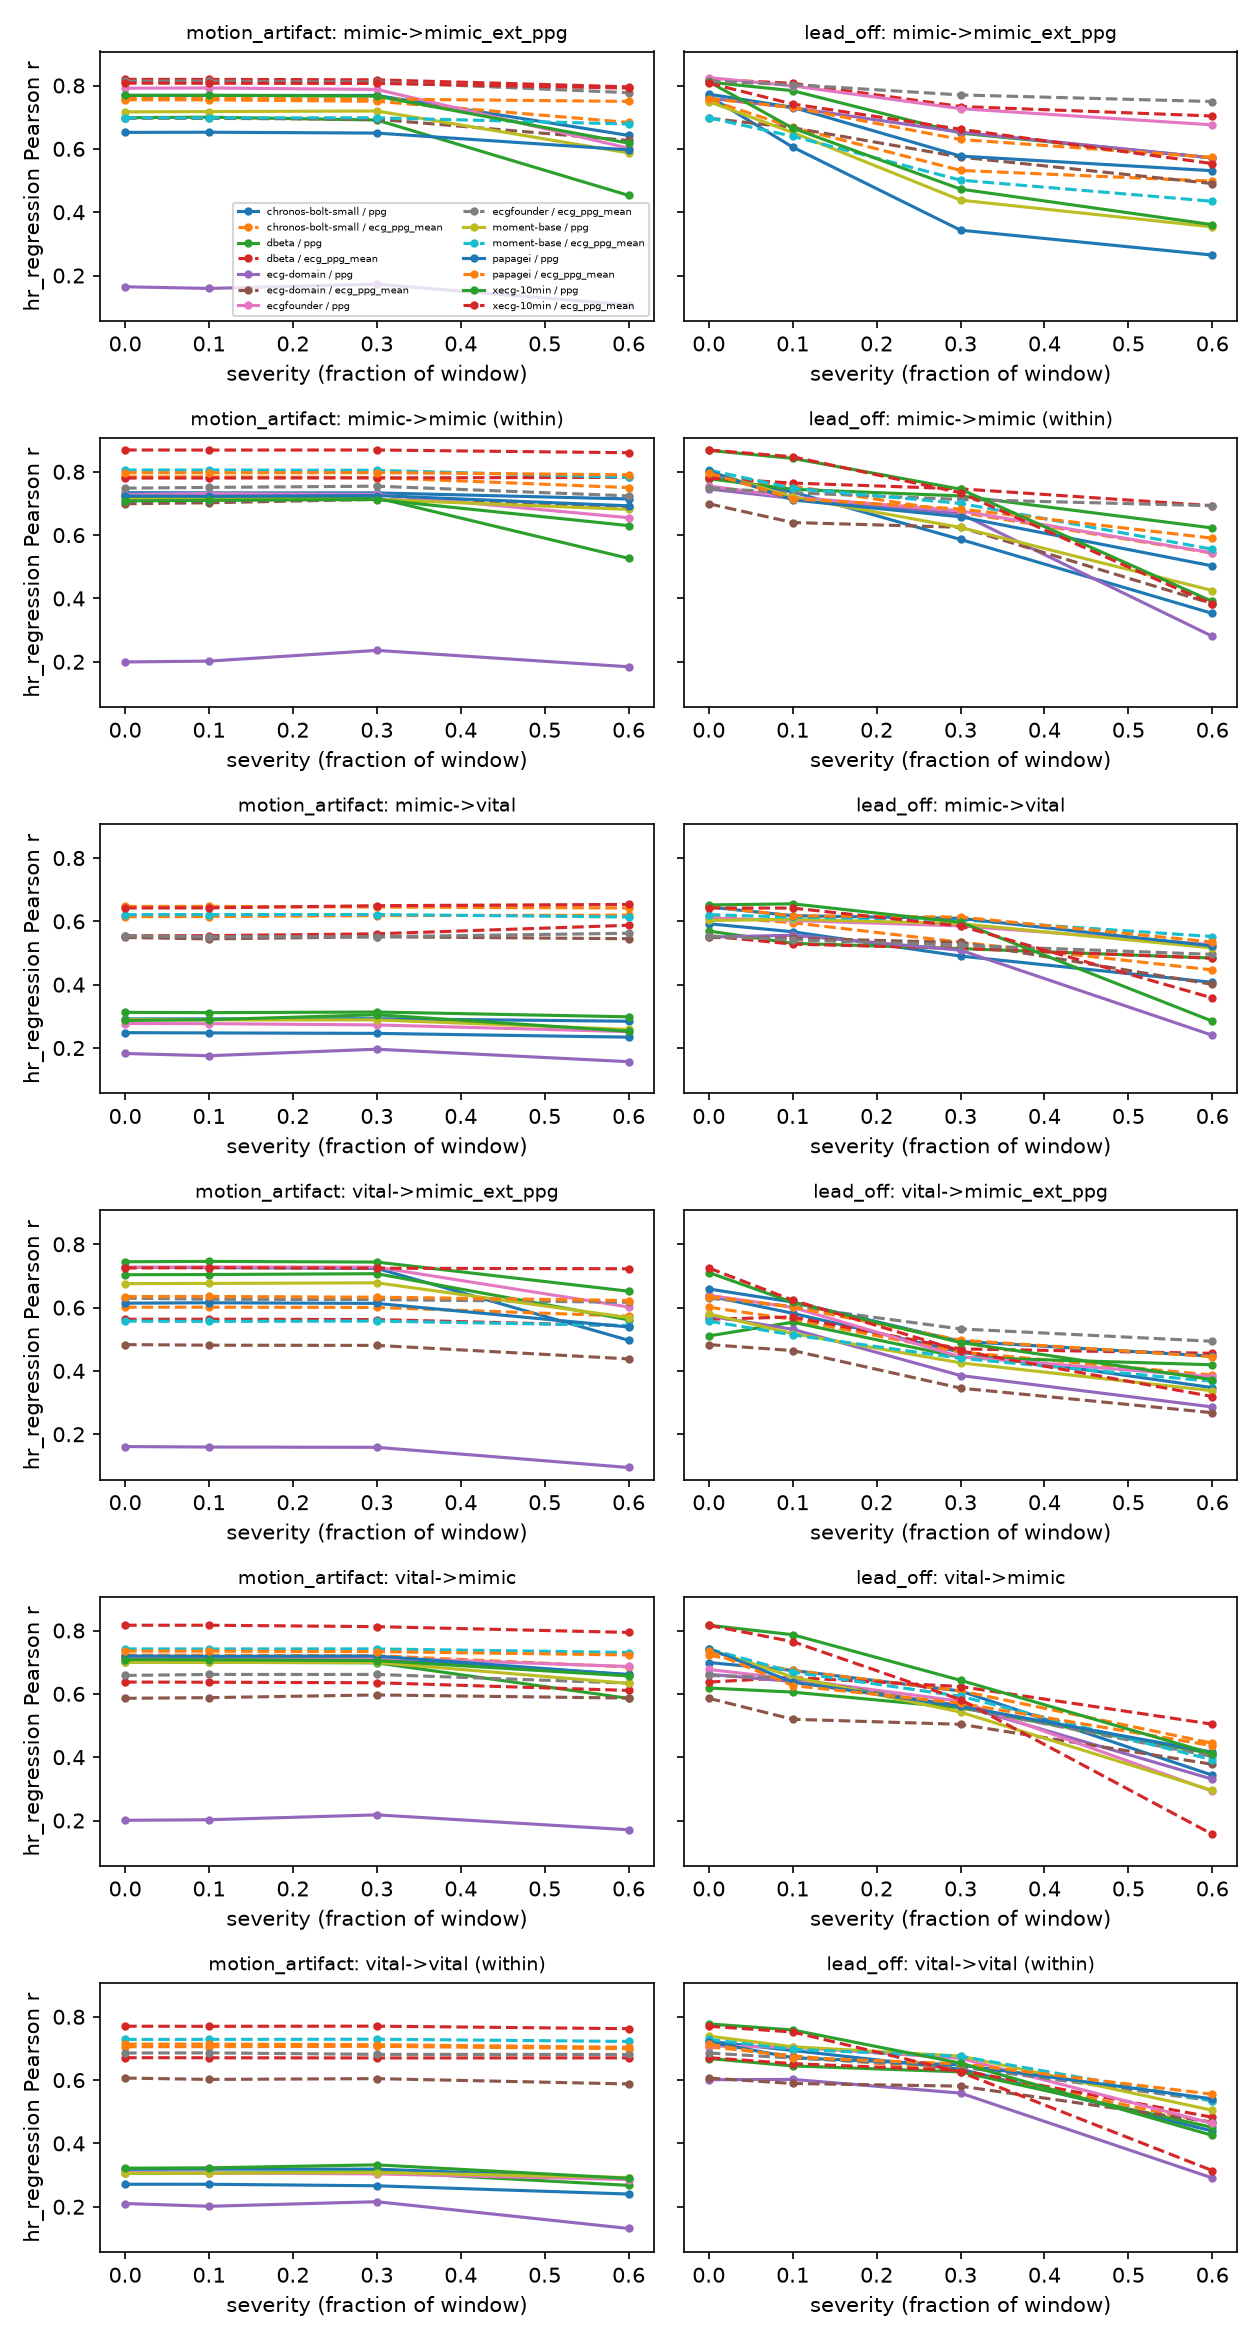
\includegraphics[height=0.62\textheight]{figures/fig2a_severity_curves_hr_regression.png}}
\end{figure*}

\begin{figure*}[t]
\floatconts
  {fig:coverage}
  {\caption{Share of the summed positive heart-rate harm that falls in windows flagged by each label-free rule and by the supervised detector, per fault, severity, and affected probe, averaged over encoders and PulseDB source--target pairs. Black ticks give the fraction of windows whose estimate moves by more than 5 beats per minute. The two cells with material harm and low coverage are the one-second lead-off cells.}}
  {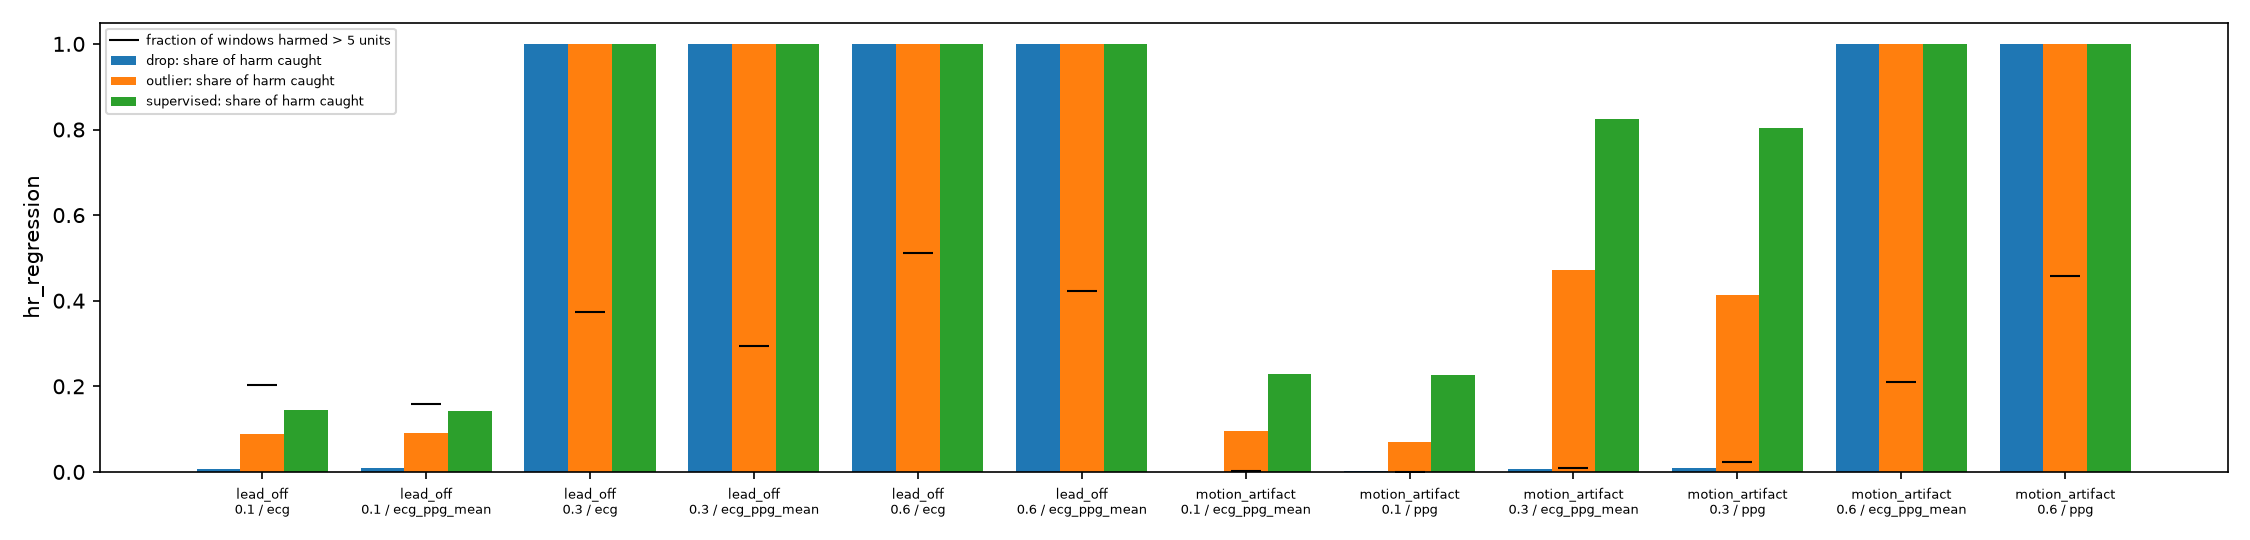
\includegraphics[width=\linewidth]{figures/fig2d_harm_coverage_hr_regression.png}}
\end{figure*}

\subsection{Label-free clustering separates only severe faults, supervision separates moderate ones, and cross-institution shift has no fingerprint}
\label{sec:taxonomy_results}

Clustering the quality and disagreement features without labels recovers the two synthetic fault classes when they are severe and nothing else (\tableref{tab:taxonomy}). With $k=3$ and the source database withheld, severity-0.6 lead-off windows land in a cluster of their own with recall 0.99 (95\% CI $[0.98,1.00]$; $n=6{,}473$) and severity-0.6 motion windows with recall 1.00 ($[1.00,1.00]$), with 54 and 136 cross-assignments between the two. Severity-0.1 and 0.3 windows of both kinds, 12,728 lead-off and 12,794 motion windows, fall into the third cluster together with 2,053 of the 2,093 structural windows, so recall at those severities is at most 0.02 and the structural class is never named (\figureref{fig:confusion}). Withholding the disagreement feature or keeping only the quality features changes no recall by more than 0.01; including the source database does not change the synthetic recalls and cannot make structural windows a cluster, because the class is defined by that column.

Supervision shows that the moderate faults are separable and the mild ones are not. Gradient-boosted trees under subject-grouped cross-validation recover lead-off with recall 0.04, 1.00, and 1.00 at the three severities and motion with 0.45, 0.97, and 1.00, and logistic regression 0.01, 0.99, and 0.99 and 0.32, 0.91, and 1.00 (\tableref{tab:taxonomy}). The clustering's failure at severity 0.3 is therefore an allocation limit of $k=3$ rather than a feature limit. Detecting first and clustering only the detected windows closes the gap for lead-off but not for motion: the drop rule flags 100\% of severity-0.3 lead-off, the silhouette selects $k=3$, and the clusters separate by flat-line duration into a 2-second and a 5-second ECG class and a 6-second PPG class, giving overall recall 0.99 at severity 0.3; the same rule flags 5\% of severity-0.3 motion, so its overall recall stays at 0.01 (\appendixref{apx:taxonomy}).

Clean windows from the second institution carry no fingerprint. Out of fold, the supervised binary classifier separates clean Seoul from clean Boston windows with an AUROC of 0.68 on all label-free features and 0.67 on the quality features alone, and the disagreement statistic alone gives 0.62 ($n=2{,}093$ versus $1{,}980$); with the source database included the AUROC is 1.00, which is circular. In the three-class supervised fit the structural prediction behaves as a no-fault class: 77\% of clean Boston controls are assigned to it. The cross-institution PPG heart-rate loss of \sectionref{sec:tasks} is therefore real and shared by every encoder, and it is invisible to a per-window quality index and to the disagreement of two probes trained on the source institution.

The taxonomy transfers to real degradation in proportion to how far the real faults resemble the injected ones. Assigned to the nearest $k=3$ centroid, 13.6\% of BUT PPG's 3,058 unusable recordings land in the motion cluster against 7.6\% of its 830 usable ones. Under the drop rule, 31.8\% of the unusable and 17.2\% of the usable recordings are flagged, 5.1\% of MIMIC-III-Ext-PPG's natively poor-PPG segments against 0.1\% of its natively clean ones, and 2.4\% of its poor-ECG segments; 0.1\% of clean Boston controls are flagged. The human usability label of BUT PPG is itself only weakly related to measured noise, with accelerometer dynamics separating the two labels at an AUROC of 0.57 (\sectionref{sec:degradation}), so a rule calibrated to injected faults is not expected to reproduce it (\figureref{fig:severity_recall}).

\begin{table*}[t]
\floatconts
  {tab:taxonomy}%
  {\caption{Recall of each known condition by injected severity, with the source database withheld from the features. Clustering is $k$-means with $k=3$ on all fit windows, named by majority vote; two-stage is the drop rule followed by clustering of the flagged windows with silhouette-chosen $k$ (detection rate and overall recall); supervised is out-of-fold recall under subject-grouped five-fold cross-validation. Brackets are subject-clustered bootstrap 95\% confidence intervals; $n=6{,}473$ windows per synthetic cell and $2{,}093$ structural windows. The supervised structural recall is the share of clean Seoul windows assigned to the structural class, to which 77\% of clean Boston controls are also assigned.}}%
  {\footnotesize\setlength{\tabcolsep}{3pt}
  \begin{tabular*}{\linewidth}{@{\extracolsep{\fill}}llcccccc@{}}
  \toprule
  & & & \multicolumn{2}{c}{\textbf{Two-stage}} & \multicolumn{2}{c}{\textbf{Supervised}} \\
  \cmidrule(lr){4-5}\cmidrule(lr){6-7}
  \textbf{Condition} & \textbf{Severity} & \textbf{$k$-means, $k=3$} & \textbf{Detected} & \textbf{Recall} & \textbf{Boosted trees} & \textbf{Logistic} \\
  \midrule
  Lead-off & 0.1 & 0.00 [0.00, 0.00] & 0.02 & 0.01 & 0.04 [0.03, 0.04] & 0.01 [0.01, 0.01] \\
  Lead-off & 0.3 & 0.02 [0.01, 0.02] & 1.00 & 0.99 & 1.00 [1.00, 1.00] & 0.99 [0.98, 1.00] \\
  Lead-off & 0.6 & 0.99 [0.98, 1.00] & 1.00 & 1.00 & 1.00 [1.00, 1.00] & 0.99 [0.98, 1.00] \\
  Motion artifact & 0.1 & 0.01 [0.00, 0.02] & 0.02 & 0.01 & 0.45 [0.42, 0.49] & 0.32 [0.29, 0.35] \\
  Motion artifact & 0.3 & 0.01 [0.00, 0.03] & 0.05 & 0.01 & 0.97 [0.97, 0.98] & 0.91 [0.89, 0.93] \\
  Motion artifact & 0.6 & 1.00 [1.00, 1.00] & 1.00 & 1.00 & 1.00 [1.00, 1.00] & 1.00 [1.00, 1.00] \\
  Structural & -- & 0.00 [0.00, 0.00] & 0.02 & 0.00 & 0.77 [0.67, 0.86] & 0.86 [0.79, 0.93] \\
  \bottomrule
  \end{tabular*}}
\end{table*}

\begin{figure}[t]
\floatconts
  {fig:confusion}
  {\caption{Cluster assignment versus known condition for $k$-means with $k=3$, all features except the source database. Cells give the column-normalized share and the count. The unnamed cluster holds every structural window and every mild and moderate synthetic window.}}
  {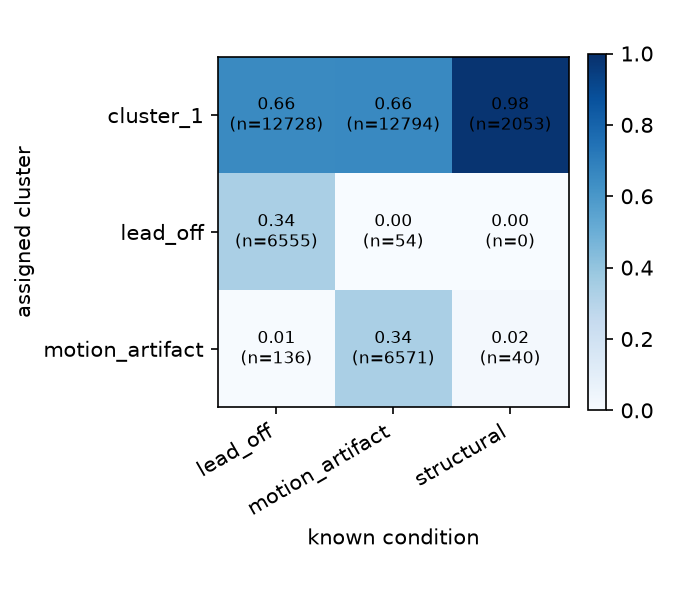
\includegraphics[width=\linewidth]{figures/fig3b_confusion.png}}
\end{figure}

\begin{figure}[t]
\floatconts
  {fig:severity_recall}
  {\caption{Recall of the own-named cluster by injected severity for the two synthetic faults, $k$-means with $k=3$, with subject-bootstrap 95\% confidence intervals. Both faults are recovered at severity 0.6 and neither below it.}}
  {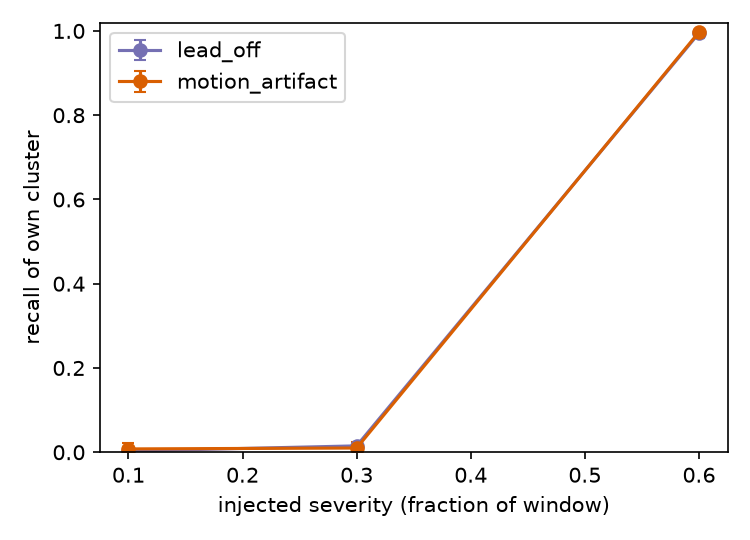
\includegraphics[width=\linewidth]{figures/fig3e_severity_recall.png}}
\end{figure}

\section{Discussion}
\label{sec:discussion}

We re-measure a single-site ranking of biosignal foundation models across two institutions and under injected sensor faults, and we test whether the faults that hurt can be seen without labels. The ranking transports and the class-level claim does not: one domain model leads, the general time-series models beat the other domain models, heart rate transports and blood pressure does not, and mean fusion never beats the better single modality. Motion artifact at realistic levels does no harm, and a per-second quality rule catches all of the harm done at the extreme. Electrode dropout harms from one second, reorders the encoders, and is missed below three seconds by a detector whose one-second bins are the reason. Cross-institution shift leaves no per-window fingerprint.

The transport result bears on how benchmark claims about model classes should be read. If a ranking is stable across institutions while the class ordering fails at both, the single-site claim was true of the checkpoints compared there and not of the classes; \domainmodel{}'s lead is a property of one model. An alternative explanation is that the single-site benchmark's tasks or fine-tuning regime favored its domain models in ways our frozen-embedding, three-task protocol does not reproduce, and we do not evaluate its rhythm task. What the evidence supports is that under an identical linear-probe protocol at two institutions, two general models outrank three of four domain models, and that heart-rate rankings are the stable part of the picture.

The stress test changes what the taxonomy's limits mean. Had moderate motion harmed the probes, the label-free rules' blindness to it would have been the gap a mitigation system must fill; it does not, so for motion the quality index already covers the harmful regime. If the noise calibration is right, then a fault-aware system can wait out any motion below the noisiest 5\% of smartphone seconds and abstain above it on the strength of a per-second rule. The calibration rests on one smartphone database and a colored-noise model, and a real artifact with structure the noise model lacks, such as baseline wander from cuff inflation, could harm the probes at lower noise ratios; the evidence covers additive noise at the measured amplitudes. Lead-off is the opposite case. Its mildest form is both harmful and undetected, and the mechanism, a one-second span straddling one-second bins, is a property of the detector we fixed before running the stress test. The finding names its own repair, and the repaired detector would need the same paired test.

The structural class is the one the taxonomy cannot deliver. A model-independent, direction-specific loss in PPG heart-rate transport shows that the two institutions differ in a way that matters for the models, and no per-window quality or disagreement feature separates their clean windows above an AUROC of 0.68. If that holds beyond this institution pair, then flagging structural shift requires information a single window does not carry, such as a labeled calibration sample from the deployment site or a population-level comparison of embeddings, which is the condition under which distribution-free coverage guarantees built on exchangeability are not expected to hold \placeholder{CITE: PhysioBridge}. The two institutions differ in care setting as well as device, and the evidence does not separate those causes.

Fusion by averaging embeddings behaves as insurance rather than gain. It halves the harm of a fault in one modality and never exceeds the intact modality's probe, within or across institutions. If a system could tell which modality a fault touched, and the taxonomy does so for severe faults, then reweighting toward the intact modality would dominate averaging; the evidence supports this for the two injected faults and says nothing about learned fusion architectures, which we do not evaluate.

\section{Limitations}
\label{sec:limits}

This study uses one institution pair, so the transport findings describe Boston intensive care against Seoul surgery and a third partition would be needed to separate device from population. Encoders are frozen and probed linearly, which is the single-site benchmark's protocol and the regime in which the claim was made, and fine-tuning could change every ranking. The faults are synthetic. Motion noise is calibrated to real smartphone-PPG noise quantiles but follows a colored-noise model and is injected into the PPG only, lead-off into the ECG only, and the injected spans are contiguous; real faults mix modalities and shapes, and BUT PPG's human quality label relates only weakly to measured noise, which limits how closely any calibration can follow it. The stress cohort is 60 subjects per institution, chosen so that every window could be embedded under seven conditions by seven encoders, and its clean cross-institution scores agree with the full-cohort transport scores to within 0.045 on average over 42 cells. Heart-rate labels are derived from the ECG by peak detection rather than annotated, validated against reference heart rates as stated in \sectionref{sec:data}. MIMIC-III-Ext-PPG shares its source hospital with PulseDB-MIMIC and its native ECG quality code does not mark flat-lines, so it validates the PPG trace and not the ECG trace. The rhythm task of the single-site benchmark and the access-restricted CSFM encoder are not evaluated. No hypothesis test is applied to the transport differences; the reported intervals cover recall only.

\section{Conclusion}
\label{sec:conclusion}

A single-site ranking of biosignal foundation models survives a second institution, but the claim that domain-specific models beat general ones does not, and neither does blood-pressure estimation. Under injected faults on paired windows, realistic motion artifact is harmless and its extreme is fully caught by a label-free quality rule, while a one-second electrode dropout harms the probes, reorders the encoders, and evades the rule for a reason that names its repair. The faults a label-free quality index misses are therefore the ones that do not hurt, with that one exception, and cross-institution shift is the fault no per-window index sees.

\acks{Acknowledgments withheld for anonymous review.}

\bibliography{ref}

\clearpage
\appendix

\section{Transport by modality}
\label{apx:transport}

\tableref{tab:transportfull} gives every cross-institution score by encoder, embedding, direction, and task. Two regularities hold across encoders. Blood pressure from the ECG embedding does not transport in either direction, with correlations of 0.01 to 0.21. Heart rate from the PPG embedding transports in one direction only: fit on Seoul and scored on Boston it reaches 0.65 to 0.69 for the six foundation models, and fit on Boston and scored on Seoul it reaches 0.32 to 0.34. The fusion probe exceeds the better unimodal probe in 6 of the 42 cells.

\begin{table*}[!t]
\floatconts
  {tab:transportfull}
  {\caption{Cross-institution probe scores (Pearson correlation) by encoder, embedding, direction, and task. HR, heart rate; SBP and DBP, systolic and diastolic blood pressure. M$\to$V, fit on PulseDB-MIMIC and scored on PulseDB-Vital.}}
  {\small\setlength{\tabcolsep}{4pt}
  \begin{tabular*}{\linewidth}{@{\extracolsep{\fill}}llcccccc@{}}
  \toprule
  & & \multicolumn{3}{c}{\textbf{M$\to$V}} & \multicolumn{3}{c}{\textbf{V$\to$M}} \\
  \cmidrule(lr){3-5}\cmidrule(lr){6-8}
  \textbf{Encoder} & \textbf{Embedding} & \textbf{HR} & \textbf{SBP} & \textbf{DBP} & \textbf{HR} & \textbf{SBP} & \textbf{DBP} \\
  \midrule
  \domainmodel{} & ECG & 0.75 & 0.21 & 0.17 & 0.80 & 0.16 & 0.20 \\
   & PPG & 0.33 & 0.39 & 0.43 & 0.68 & 0.20 & 0.36 \\
   & Fusion & 0.74 & 0.39 & 0.37 & 0.80 & 0.24 & 0.36 \\
  \tsmodel{} & ECG & 0.70 & 0.06 & 0.05 & 0.75 & 0.10 & 0.14 \\
   & PPG & 0.34 & 0.35 & 0.39 & 0.68 & 0.28 & 0.37 \\
   & Fusion & 0.70 & 0.31 & 0.30 & 0.76 & 0.24 & 0.30 \\
  Chronos-Bolt & ECG & 0.69 & 0.06 & 0.07 & 0.73 & 0.11 & 0.17 \\
   & PPG & 0.34 & 0.37 & 0.40 & 0.68 & 0.31 & 0.38 \\
   & Fusion & 0.68 & 0.31 & 0.31 & 0.74 & 0.25 & 0.32 \\
  ECGFounder & ECG & 0.66 & 0.14 & 0.14 & 0.72 & 0.15 & 0.20 \\
   & PPG & 0.32 & 0.35 & 0.35 & 0.68 & 0.26 & 0.37 \\
   & Fusion & 0.63 & 0.37 & 0.35 & 0.70 & 0.28 & 0.35 \\
  PaPaGei & ECG & 0.70 & 0.01 & 0.07 & 0.76 & 0.03 & 0.17 \\
   & PPG & 0.32 & 0.31 & 0.31 & 0.65 & 0.26 & 0.30 \\
   & Fusion & 0.69 & 0.21 & 0.21 & 0.75 & 0.19 & 0.23 \\
  D-BETA & ECG & 0.61 & 0.10 & 0.15 & 0.65 & 0.09 & 0.13 \\
   & PPG & 0.33 & 0.35 & 0.35 & 0.68 & 0.30 & 0.33 \\
   & Fusion & 0.60 & 0.27 & 0.29 & 0.66 & 0.17 & 0.22 \\
  NeuroKit2 features & ECG & 0.63 & 0.02 & 0.13 & 0.70 & 0.04 & 0.20 \\
   & PPG & 0.14 & 0.09 & 0.09 & 0.22 & 0.05 & 0.11 \\
   & Fusion & 0.60 & 0.04 & 0.10 & 0.65 & 0.03 & 0.15 \\
  \bottomrule
  \end{tabular*}}
\end{table*}

\section{Fault sensitivity by encoder}
\label{apx:sensitivity}

\tableref{tab:sensitivity} gives each encoder's heart-rate correlation under lead-off for the ECG and fusion probes and under severity-0.6 motion for the PPG probe, averaged over the four PulseDB source--target pairs. The encoders' spread widens with lead-off severity: at severity 0.6 the ECG-probe correlations run from 0.29 to 0.50, and the three encoders that degrade least, PaPaGei, D-BETA, and ECGFounder, are three of the four that rank below the general models on clean windows.

\begin{table*}[!t]
\floatconts
  {tab:sensitivity}
  {\caption{Heart-rate correlation by encoder under injected faults, averaged over the four PulseDB source--target pairs. Severity 0 is the clean condition.}}
  {\small\setlength{\tabcolsep}{4pt}
  \begin{tabular*}{\linewidth}{@{\extracolsep{\fill}}lcccccccccc@{}}
  \toprule
  & \multicolumn{4}{c}{\textbf{Lead-off, ECG probe}} & \multicolumn{4}{c}{\textbf{Lead-off, fusion probe}} & \multicolumn{2}{c}{\textbf{Motion, PPG probe}} \\
  \cmidrule(lr){2-5}\cmidrule(lr){6-9}\cmidrule(lr){10-11}
  \textbf{Encoder} & 0 & 0.1 & 0.3 & 0.6 & 0 & 0.1 & 0.3 & 0.6 & 0 & 0.6 \\
  \midrule
  \domainmodel{} & 0.78 & 0.76 & 0.66 & 0.38 & 0.77 & 0.75 & 0.63 & 0.30 & 0.51 & 0.46 \\
  \tsmodel{} & 0.72 & 0.67 & 0.61 & 0.44 & 0.72 & 0.68 & 0.64 & 0.51 & 0.50 & 0.47 \\
  Chronos-Bolt & 0.70 & 0.67 & 0.58 & 0.39 & 0.71 & 0.68 & 0.61 & 0.47 & 0.51 & 0.49 \\
  ECGFounder & 0.69 & 0.67 & 0.63 & 0.46 & 0.66 & 0.65 & 0.61 & 0.53 & 0.51 & 0.47 \\
  PaPaGei & 0.73 & 0.66 & 0.62 & 0.50 & 0.72 & 0.66 & 0.63 & 0.53 & 0.49 & 0.46 \\
  D-BETA & 0.66 & 0.63 & 0.60 & 0.49 & 0.66 & 0.65 & 0.63 & 0.54 & 0.51 & 0.42 \\
  NeuroKit2 features & 0.64 & 0.63 & 0.57 & 0.29 & 0.61 & 0.57 & 0.56 & 0.41 & 0.20 & 0.16 \\
  \bottomrule
  \end{tabular*}}
\end{table*}

\section{Taxonomy details}
\label{apx:taxonomy}

\paragraph{Cluster structure.}
With $k=3$ on all fit windows, the two named clusters are the severity-0.6 windows of each fault and the third cluster is everything else: 12,728 of 19,419 lead-off windows, 12,794 of 19,419 motion windows, and 2,053 of 2,093 structural windows. A three-cluster solution cannot split a class whose members differ only in degree from clean windows, which is what the mild and moderate severities are under a 10-second summary: a 1- to 3-second fault leaves the window's mean quality near 1 and its longest low-quality run near 0 or 1 second.

\paragraph{Two-stage clustering.}
Detecting first changes what the clusters separate. Under the drop rule, 20,095 of the 40,931 fit windows are flagged, and the silhouette selects $k=3$ for three of the four feature sets and $k=4$ for the quality features alone. The three clusters are a 2-second ECG flat-line class holding 6,404 of the 6,473 severity-0.3 lead-off windows, a 5-second ECG flat-line class holding 6,442 of the severity-0.6 lead-off windows, and a 6-second PPG drop-out class holding 6,455 of the severity-0.6 motion windows; two clusters therefore share the name lead-off. Overall recall, the product of detection rate and typing recall, is 0.99 and 1.00 for lead-off at severities 0.3 and 0.6 and 1.00 for motion at 0.6. The rule flags 352 of 6,473 severity-0.3 motion windows, because the 75th-percentile noise does not push the per-second PPG quality below 0.5, so that class stays at 0.01. Under the outlier rule 24,638 windows are flagged, including 44\% of severity-0.3 motion, but those windows form a cluster of their own only for the quality-only feature set at $k=5$ (recall 0.44) and are otherwise merged with the 2-second lead-off class. Severity-0.1 windows of both faults share one cluster in every configuration, so their recalls record only which name that cluster draws. The outlier rule is also device-confounded on smartphone PPG: it flags 77\% of BUT PPG's usable recordings and 81\% of its unusable ones against clean-monitor controls, so its held-out shares are not reported.

\paragraph{Held-out assignment.}
Under $k=3$, clean Boston controls and natively clean MIMIC-III-Ext-PPG segments are assigned to the unnamed cluster without exception (1,980 of 1,980 and 800 of 800). Of BUT PPG's unusable recordings, 417 of 3,058 land in the motion cluster, against 63 of 830 usable ones; 18 of 800 natively poor-ECG segments land in the lead-off cluster and 11 of 800 natively poor-PPG segments in the motion cluster.

\paragraph{Calibration negative result.}
Accelerometer magnitude in BUT PPG is reported in milli-g, so its mean absolute value is gravity, and its dynamics carry no information about the human usability label (AUROC 0.57) or about measured PPG noise (Spearman $-0.11$, $n=3{,}795$). A calibration that mapped severity to accelerometer range therefore collapsed to its floor and was replaced by the quantile anchoring of \sectionref{sec:degradation}.

\end{document}
